\documentclass[a4paper,12pt]{scrartcl}

\usepackage[utf8]{inputenc}
\usepackage[T1]{fontenc}
\usepackage{url}
\usepackage{fancyhdr}
\usepackage[acronym]{glossaries}
\usepackage{listings}
\usepackage{amsmath}
\usepackage{amssymb}
\usepackage{graphicx}

\usepackage[mathcal]{euscript}

\usepackage[
	backend=biber,
	style=alphabetic,
	sorting=ynt
]{biblatex}
\addbibresource{references.bib}

\fancyhead[R]{}
\fancyhead[C]{The BLS Signature Scheme}
\fancyhead[L]{}

\pagestyle{fancy}
\renewcommand{\headrulewidth}{0.5pt}

\fancyfoot[C]{\thepage}
\renewcommand{\footrulewidth}{0.5pt}

\begin{document}

\begin{titlepage}
\begin{center}
\vspace*{3cm}
\vspace{1cm}
\Huge \textbf{The BLS Signature Scheme} \\
\vspace{6cm}
\vspace{1cm}
\large Gabor Tanz \\ gabor.tanz@students.bfh.ch \\
\end{center}
\end{titlepage}

\tableofcontents
\pagebreak

\begin{abstract}
	This document explains the BLS signature scheme and the necessary mathematic basics and one of its uses for cryptocurrencies.
\end{abstract}
\pagebreak

\section{Introduction}
\pagebreak

\section{Prerequisites}
The following mathematical concepts are needed to better understand how the BLS Signature scheme works.
\subsection{Abstract Algebra}
Abstract Algebra deals with abstract structures rather than number systems. The structures that are relevant for this paper are groups and fields.
\subsubsection{Group Theory}

\paragraph{Definition}\hfill

A group is a set with a binary operation $\circ$, so that two elements of the group produce another element of the group and a unary operation $inv$ that inverses $\circ$.

The operation needs to satisfy the following properties.
\begin{itemize}
	\item Associativity, which means the order of operations doesn't matter
	\item Identity, an identity element $e$ exists, so that $\circ$ with any element of the group and the identity element produces the element itself.
	\item Inverse, for each element $a$ in $G$ there exists an inverse element $b$, so that the two produce the identity element $e$.
	\item Closure, for any element in $G$ the result of the operation $\circ$ is also in $G$. This is implied by satisfying the other three properties.
\end{itemize}

\paragraph{Mathematical definition}\hfill

Group: $\mathcal{G} = (G, \circ, inv, e)$

Associativity: $ x \circ (y \circ z) = (x \circ y) \circ z$ $\forall x,y,z \in G $

Identity: $ e \circ x = x \circ e = x $ $ \forall x,e  \in G $

Inverse: $ x \circ inv(x) = inv(x) \circ x = e $ $ \forall x \in G $

Closure: $ \forall x,y \in G \rightarrow x \circ y \in G $

\paragraph{Examples}\hfill

The set of integers $\mathbb{Z}$ with the operation $+$, the identity element 0 and the inverse operation $-$. $\mathcal{G} = (\mathbb{Z},+,-,0)$

The set of integers $\mathbb{Z}$ modulo $n$ with the operation $\times$, the identity element 1 and the inverse operation $^{-1}$. $\mathcal{G} = (\mathbb{Z}_{n}^*, \times_{n}, ^{-1}, 1)$

\subsubsection{Cyclic Groups}

A group is cyclic if it can be generated by a single element x (the generator). We will just focus on groups modulo $n$ as they are the most relevant in cryptography. In a group modulo $n$ the order of an element $x\in G$ is noted by ord($x$). It is the smallest $k$ > 0, such that $x^k = 1$ mod n.

$g\in G$ is a generator for the finite group $\mathcal{G} = (G, *, ^-1, 1)$ if ord($g$) = ord($\mathcal{G}$). A generator $g$ needs to be a primitive root modulo $n$.

\paragraph{Examples}

3 is a generator of $\mathbb{Z}_7^*$. The powers of 3 mod 7 are 3,2,6,4,5,1, which are all elements in $\mathbb{Z}_7$.

2 is not a generator of $\mathbb{Z}_7^*$. The powers of 2 mod 7 are 2,4,1, which aren't all elements in $\mathbb{Z}_7$.

As at least one element in $\mathbb{Z}_7$ exists that can generate the group it is cyclic.

$\mathbb{Z}_4^*$ is not a cyclic group as none of the elements can generate the group.

\subsubsection{Fields}

A field is based on a set and two operations, which each set/operation combination forming abelian or commutative groups, further both operations are distributive.

The field $(K, +, *)$ is based on the two abelian groups $(K, +, -, 0)$ and $(K\\0, *, ^-1, 1)$. Distributivity is defined as: $\forall a,b,c\in K$: $a*(b+c) = a*b+a*c, (a+b)*c = a*c+b*c$.

\paragraph{Example}

An example for a finite field is $(\mathbb{Z}$ mod 5 $, +, -, 0, *, ^{-1}, 1)$, which consists of the groups $(\mathbb{Z}$ mod 5 $, +, -, 0)$ and $(\mathbb{Z}$ mod 5 $, *, ^{-1}, 1)$.


\subsection{Elliptic curves (EC)}
\subsubsection{Definition}
An elliptic curve is a set of points \((x,y)\) satisfying the equation:
\begin{equation*}
y^2 = x^3 + ax + b
\end{equation*}

The elliptic curve is defined over a field $\mathbb{F} = (F, +, -, 0, *, ^{-1}, 1)$ such that $4a^{3} + 27b^{2} \neq 0$.
The resulting points for a set $E_a,b (F)$ that is defined as: ${(x,y) \in F \times F: y^{2} = x^{3} + ax + b}$ $\cup$ $\{\mathcal{O}\}$, where $\mathcal{O}$ is called the point of infinity.

\begin{figure}[hbt!]
	\centering
	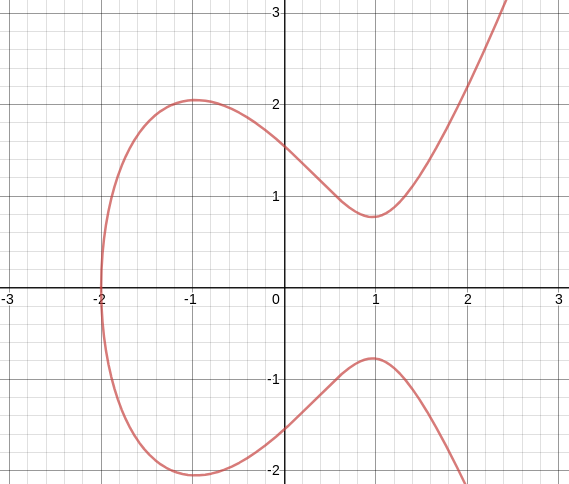
\includegraphics[width=0.5\linewidth]{ec1}
	\caption[]{Example of an elliptic curve: $y^2 = x^3 - 2.8x + 2.4$}
	\label{fig:ec-b2}
\end{figure}


Every line that intersects the curve does it at exactly 3 points. If a point is tangent to the curve it is counted twice, if the line is vertical the point at infinity is also counted. With this property a binary operation + and an unary operation - on curve points can be defined, which form an additive Group $\mathcal{G} = (E_a,_b (F), +, -, \mathcal{O})$.

The additive inverse of a curve Point $P$ is defined as $\mathcal{O}$ if $P$ is $\mathcal{O}$ and mirrored on the x-Axis otherwise:
\[
-P =
\begin{cases}
\mathcal{O} & \text{, if } P = \mathcal{O} \\
(x,-y) & \text{, if } P = (x,y)
\end{cases}
\]

\subsubsection{Addition of curve points}
The addition of two curve points $P$ and $Q$ is defined as the mirror on the x-Axis of the 3rd intersection point $R$:
\[
P+Q =
\begin{cases}
\mathcal{O} & \text{, if } P = -Q \\
P & \text{, if } Q = \mathcal{O} \\
Q & \text{, if } P = \mathcal{O} \\
-R & \text{, if } P \neq -Q \text{ and } P,Q \neq \mathcal{O}
\end{cases}
\]

\begin{figure}[hb!]
	\centering
	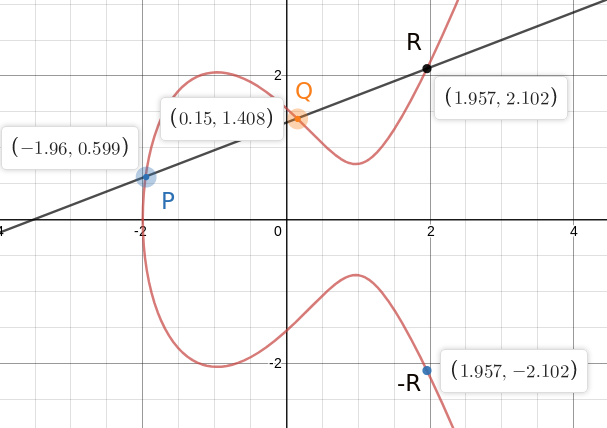
\includegraphics[width=0.5\linewidth]{ec2}
	\caption[]{Example with $P, Q, R$ and $-R$}
\end{figure}

If we look at the "normal" case where $P$ isn't $-Q$ and neither $P$ nor $Q$ are $\mathcal{O}$, we can define the addition as follows:
\[ P = (x_1,y_1), Q = (x_2,y_2) \]
\[ P + Q = (x,y) = (m^2 - x_1 -x_2, m \times (x_1 - x) - y_1) \]
\[ m =
\begin{cases}
\frac{y_2 - y_1}{x_2 - x_1}
& \text{, if } P \neq Q \\
\frac{3x_1^2 + a}{2y_1}
& \text{, if } P = Q
\end{cases}
\]

\subsubsection{Elliptic curves over finite fields}
A finite field can be given by $(\mathbb{Z}_p,+,-,0,\times,^{-1},1)$ if $p$ is prime. When an elliptic curve is defined over this field the points are finite(they repeat) but the behaviour is otherwise normal, it would be written as $E_a,_b (\mathbb{Z}_p)$.

Example: $E_2,_5 (\mathbb{Z}_7)$ for $y^2 \equiv x^3 + 2x + 5$ mod $7$.
\begin{align}
(1,1) \in E_2,_5 (\mathbb{Z}_7) & \text{ because } 1^2 \equiv 1^3 + 2\times{1} + 5 \text{ mod } 7 \\
(4,0) \in E_2,_5 (\mathbb{Z}_7) & \text{ because } 0^2 \equiv 4^3 + 2\times{4} + 5 \text{ mod } 7 \\
(2,2) \notin E_2,_5 (\mathbb{Z}_7) & \text{ because } 2^2 \not \equiv 2^3 + 2\times{2} + 5 \text{ mod } 7 
\end{align}
$E_2,_5 (\mathbb{Z}_7) = \{ (1,1),(1,6),(4,0),(5,0),(6,3),(6,4), \mathcal{O} \}$

\begin{figure}[hbt!]
	\centering
	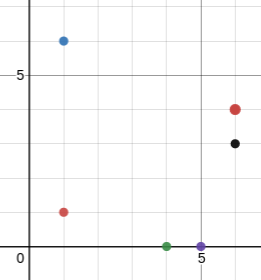
\includegraphics[width=0.5\linewidth]{ec3}
	\caption{$y^2 \equiv x^3 + 2x + 5$ mod $7$}
\end{figure}

Addition works with the same formula as before, but because we are operating on a finite field, we can create a table for all possible additions as they will repeat themselves. In elliptic curves over a finite field every point is a generator if the order of the curve is prime.

\subsection{Bilinear Maps}
A bilinear mapping $e$ maps two additive cyclic groups $G_1$ and $G_2$ of the same prime order $q$ to the multiplicative group $G_t$ of order q. For a pairing function $e$ to be bi-linear, it has to satisfy these properties:
\begin{itemize}
	\item commutativity for additive and multiplicative operations
	\item distributivity for multiplicative operations
\end{itemize}
\[ e: G_1 \times G_2 \rightarrow G_t \]
such that
\[ \forall a,b \in \mathbb{Z}, u \in G_1, v \in G_2: \]
\[ e(u^a,v^b) = e(u,v)^ab \]

This means that $e(u^a,v^b) = e(u^b,v^a)$ as $e(u,v)^ab = e(u,v)^ba$.

\begin{figure}[hbt!]
	\centering
	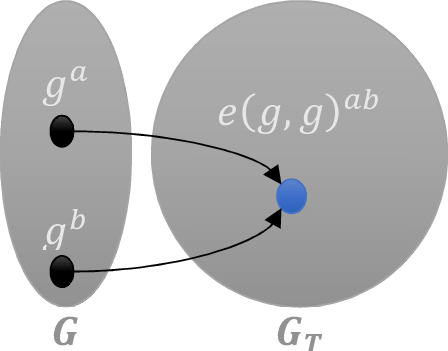
\includegraphics[width=0.5\linewidth]{pairing1}
	\caption{illustration of pairing}
\end{figure}

Another important property of this pairing is that it is non-degenerate, which means that if $u$ and $v$ are generators of $G_1$ and $G_2$ then $e(u,v)$ generates $G_t$, otherwise $e = 1$ would be a valid paring.
Usually $G_1 = G_2$ so it will be noted as $G$ from now on.

In our example the source Group $G$ are the points of an Elliptic Curve and the target Group is a multiplicative subgroup of a finite field.
\[ G \subseteq E(F_p) \]
\[ G_t \subseteq (F_p \alpha)^{*} \]
\[ ( \alpha = 1, 2, 3, 4, 6, 10, 12 ) \]

\pagebreak

\section{BLS Signatures}
\subsection{Signature Schemes}

A signature scheme is used for verifying the authenticity of digital messages. With a signature a recipient can verify that a message was sent by the sender it claims(authentication) and that it wasn't tampered with(integrity).

A Signature scheme uses the following 3 algorithms:
\begin{itemize}
	\item key generation
	\item signature generation
	\item signature validation
\end{itemize}

In most cases the signature is applied on the hash of the message instead of the message itself, as the calculation of the signature is often slow and the signature size depends on the message size. 

\subsubsection{Key generation}

The key generation algorithm generates a keypair consisting of a private and public key. The private key needs to be selected uniformly at random. It should not be possible to generate the private key with knowledge of the public key. Formally the key generation function is called $G$ and takes a security parameter $n$ and generates a secret key $sk$ and a public key $pk$.
\[
G(n) := sk \text{ and } pk.
\]

\subsubsection{Signature generation}

The signature generation algorithm takes the message and the private key as input and generates a signature. Formally the function is called $S$ and takes the secret key $sk$ and the message $m$ as input and generates a tag $\sigma$.
\[
S(sk, m) := \sigma
\]

\subsubsection{Signature validation}

A signature can be validated with the message and the public key. The algorithm either accepts or rejects. Formally the function is called $V$, which takes the inputs $pk$, $m$ and $\sigma$.
\[
V(pk, m, \sigma) := \text{ true or false}
\]

\subsubsection{Hash functions}

A hash function generates for a message of arbitrary size a value of fixed size, called hash. It should not be possible to reconstruct the message from the hash and the same input should always produce the same output. This way the integrity of a message can be verified.

\subsection{The BLS Signature Scheme}
The BLS Signature Method (named after Boneh, Lynn and Shacham) uses bi-linear pairing with an elliptic curve group.
Formally we have the following functions defining the scheme.
\begin{itemize}
	\item Key generation $G()$
	\begin{center}
		random \( x\in \mathbb{Z}_{q} \) and set \( h \leftarrow g_{1}^\alpha\in \mathbb{G}_{1} \) output: \( pk := \)(h) and \( sk := (\alpha) \)
	\end{center}
	\item Signature generation $S(sk, m) $
	\[ \sigma\ := h^x  h := H(m) \]
	\item Singature validation $V(pk, m, \sigma)$
	\begin{center}
		if \( e(g_{1},\sigma) = e(pk, H_{0}(m)) \) accept, otherwise reject
	\end{center}
\end{itemize}

Interesting properties of the BLS Signature scheme are
\begin{itemize}
	\item threshold signature and key generation
	\item signature aggregation
\end{itemize}

\subsection{Threshold Signatures}

In a threshold cryptosystem a valid signature can be generated if a number of participants, larger than the threshold $n$, contribute a signature share into an overall signature. This signature is valid as if all participants had signed the message.

\subsection{Blind Signatures}

\pagebreak

\section{BLS Signatures and for Cryptocurrencies}
\subsection{Secret Sharing}
Shamir secret sharing https://blog.dash.org/secret-sharing-and-threshold-signatures-with-bls-954d1587b5f
\subsection{Cryptocurrencies}
\subsubsection{Advantages}
\begin{itemize}
	\item short Signatures
	\item aggregation of signatures and keys
\end{itemize}

\subsubsection{Uses}
\begin{itemize}
	\item Dashpay
\end{itemize}

\subsection{Blinding}
Given signature \( \langle \sigma, g^x \rangle \) on message \( h \), we can blind the signature and public key \( g^x \):
\[ e(\sigma^b,g) = e(h,g)*{xb} = e(h,g^{xb}) \]
Thus \( \sigma^b \) is a valid signature for the derived public key \( (g^x)^b \) with blinding value \( b \in \mathbb{Z}_{q} \).\cite[PKI Slide 12]{crypto-slides-grothoff}
\pagebreak

\section{Conclusion}

\printbibliography

\end{document}
